\documentclass[12pt]{memoir}
\usepackage{common}

\addbibresource{references}

\title{}
\author{Andrew Head}

\begin{document}

\definition{Title}{Understanding and Improving Student Engagement and Reuse with In-the-Wild Programming Examples}

\definition{Author}{Andrew Head, PhD Student, UC Berkeley}

\definition{Keywords}{code examples; code reuse; informal education;}

%%% Introduction

Recently, comprehensive~\cite{parnin_crowd_2012}, high-quality~\cite{mamykina_design_2011} crowd-developed online documentation has made it easier than ever for programmers to fall back on the web to find examples of how to use unfamiliar language features and APIs~\cite{brandt_two_2009}.
But using online documentation can be fraught with hazards.
When learning just the bare minimum to do a coding task (i.e., programming ``opportunistically''~\cite{clarke_what_2007}), programmers develop shoddy code that just satisfies the intended functionality, reimplement code that stable libraries could support, and spend time debugging code~\cite{brandt_opportunistic_2008,brandt_two_2009}.

A CS student's upper division courses and project work often offers them their first opportunities to satisfy information needs to using these online sources almost exclusively.
And while code examples have been identified as a critical component of CS education~\cite{lahtinen_study_2005}, we do not understand the role of the online code example in upper division programming learning.
One reason is that online code examples have only recently become available to programmers on a large scale and with reliable quality, in many ways in part to the creation of StackOverflow, a massive, popular programming Q\&A, launched in 2008.

Several important questions about the role of the online code example in non-formal learning are significant to improving CS Education in upper division courses and the ability of newly-graduated programmers to learn on the job.
These questions include:
When copying and pasting is easy, do programmers actually learn new concepts from code examples ($Q1$), e.g., enough to design new code from the same components ($Q2$)?
How often do they reuse code that contains bugs, style errors, or non-idiomatic code ($Q3$)?
How long does this code remain in use ($Q4$)?
What interventions can supplement information seeking to encourage successful learning ($Q5$)?
What interfaces can support more successful reuse of code found online ($Q6$)?

%%% Problem statement

My proposed research seeks to \textbf{understand the affordances and pitfalls of student programmers working with online code examples for informal learning, to categorize and count the mistakes made, the frequency of knowledge gained, and the opportunities to build interventions in the form of novel interfaces that can to enable students to effectively work with and benefit from online examples.}

%%% The Approach

I can gain deeper, generalizable insight on each of these questions by following standard techniques of observation and systems evaluation from HCI\@.
In each case, the critical question to the design of my research is \emph{how can I simulate scenarios of web-based code reuse in a controlled setting, and measure behavior with code examples?}
While a variety of techniques are available, I can offer the most knowledge to the academic community by observing reuse habits in two ways.
First, I will conduct controlled lab studies to address $Q1-4$, (e.g.,~\cite{ichinco_exploring_2015,brandt_two_2009,head_tutorons_2015}) with dozens of participants sampled from Berkeley's large population of EECS undergraudate students.
Second, I will conduct contextual inquiry~\cite{beyer_contextual_1997} with members of student groups during implementation prototypes for Berkeley's upper division user interface course, a period where discovery and testing of user interfaces within a team are likely at their prime.

Given this knowledge, I will develop a new generation of web and IDE-based interventions for better supporting learning and reuse from online code examples.
This body of systems will satisfy, I suspect, two major needs:
First, the need to support better understanding of code found in the wild at lower cost via automatic explanations.
This is a need we have already address with the Tutorons infrastructure I built for past work and will be easily adaptable to the problem at hand~\cite{head_tutorons_2015}.
Second, the need to support new forms of mental model-building, learning and interaction with code examples.
Once again, this can be gained supported with in-situ, in-the-browser interactions akin to those.
However, there are challenges to both building automatic help and providing it in a form that will be instantly read within the browser.
We propose that interactions that force close inspection of code prior to pasting will enable better design with these components later on down the road.
We will use standard techniques to measure the quality of code produced (e.g.,~\cite{brandt_example-centric_2010}), ability to process code found anywhere (e.g.,~\cite{head_tutorons_2015}), and user ability to complete tasks with the interface (e.g.,~\cite{head_tutorons_2015}).
The result will be a set of concrete software artifacts and an understanding of how these new interactions better support learning and reuse of code.

%%% Intellectual Merit

Surprisingly little is known about these questions.
Recent work has shown reliance on example reuse for end-user programmers~\cite{brandt_two_2009}, as well as hurdles and strategies for complete novices~\cite{ichinco_exploring_2015}.
It is clear from my experience debugging code with students as a student instructor that reuse occurs frequently in the upper division CS classroom, and that hastily pasted code is the cause of confusion and errors.
From speaking with other professors, this is no uncommon occurrence.
While a large body of work in CS Education has proposed and evaluated curricula (e.g.,~\cite{tew_developing_2010}), assignments, and textbook examples (e.g.,~\cite{borstler_quality_2011}), the online code example is an important learning resource that we don't understand.

The work we produce here will be disseminated by three major means.
Insights gathered about the challenges and strategies of programmers reusing code will be disseminated among the end-user and novice programmer communities at conferences including CHI and VL/HCC\@.
The systems, interventions, and techniques we generate will be instantiated in software artifacts and published at UIST, the premier conference in novel user interface technology.
Finally, all programming tools developed will be made open source and available for immediate public use.

%%% Broader impacts

Learning new computer science skills ``on the job'' is a core competency for both professional computer science practitioners~\cite{exter_exploring_2012} and end-user programmers in a variety of professions~\cite{dorn_learning_2010}.
As online snippets increase in quality, it is critical that we understand the something.
Developing solid mental models is one of the great challenges of taking on new work as a software engineer.
When online examples threaten to obviate the need for the right mental models to get work done, it is important that we understand the learning opportunities that are missed, the software mistakes that are introduced, and the next generation of systems that can better support the development of these mental models and responsible reuse of code.
This research will produce both this critical understanding, and will evaluate a newly-developed set of interactions to support programmers' increased reliance on the web for programming information seeking.
I have already gained interest from faculty members in the Berkeley department for conducting a lecture on responsible code reuse that could come a result of the proposed research.
This relates to the NSF broader impact of \textbf{increasing and improving public engagement with science and technology}.

\if 0

\section{Background}

Clarke introduced the persona of an \emph{opportunistic developer} to describe the software developer who develops just enough of an understanding of a technology to solve a business problem~\cite{clarke_what_2007}.
Recent studies have observed opportunistic behavior for programmers beyond business, including creative workers~\cite{brandt_opportunistic_2008} and web designers~\cite{dorn_learning_2010}.
While this style of development enables rapid results~\cite{brandt_opportunistic_2008}, it comes with hazards:
functionality is copied and pasted from online examples, with less attention to explanations~\cite{brandt_two_2009};
code may be written in a sub-optimal way in order to maintain flow and move on to other tasks~\cite{brandt_opportunistic_2008}.
% programmers are more likely to re-implement functionality instead of reusing established systems and libraries~\cite{brandt_opportunistic_2008};

Past observation confirms that the cards are stacked against typical programming documentation for maintaining the attention of those developing opportunistically.
In human-computer interaction, Carroll writes how users learning new technologies are often too busy learning to make use of instruction~\cite{carroll_nurnberg_1990}.
For end user programmers (those programming for personal purposes~\cite{ko_state_2011}), Blackwell's Attention Investment models how programmers carefully weigh the costs of engineering activities against perceived benefits~\cite{blackwell_psychological_2006}.
Good software engineering practice, like understanding the model of an API, often loses to expediency.

When a programmer's focus centers on trial and error with code instead of making sense of comprehensive references, we face two tasks to better support the opportunistic developer in understanding found code.
First, \textbf{relevant documentation should be moved from hidden locations to the code examples they arre used in.}
Second, \textbf{documentation should be provided in a context-relevant, easy-to-read, short form.}

Meanwhile, a growing corpus of online high-quality ``crowd documentation''~\cite{parnin_crowd_2012} provides new environments in which to support context-relevant documentation and new resources to mine and serve to information seekers in a context-relevant form.

\section{Proposed Research}

I hypothesize that new techniques for delivering context-relevant, summative documentation will help opportunistic developers in two ways:
\begin{itemize}[noitemsep,topsep=0pt]
\item By decreasing verbosity and increasing relevance, it will enable programmers to gain the same understanding of libraries with less effort
\item When presented next to code examples, it can lesson the effort required to develop solutions involving unfamiliar software
\end{itemize}

I propose three systems to demonstrate the potential of context-relevant, summative programming documentation.
The \textbf{intellectual merit} of the first of these systems has already been recognized:
the Tutorons work has received an Honorable Mention VL/HCC~\cite{head_tutorons_2015}, a main conference on end user programming.
Prototypes for the other systems two have been built.
They must undergo substantial further development and evaluation.

\subsection{Tutorons}
% Context-relevant descriptions of online code found during opportunistic information seeking.
Programmers often encounter syntax that they don't understand in web tutorials that has not been explained by the tutorial author.
A Tutoron is a routine on a public server that can detect code snippets in the markup for tutorial pages, and synthesize English prose, diagrams, and usage examples to describe this code.
When a programmer navigates in a browser instrumented with the Tutorons plugin, programmers can view context-relevant explanations of high-level intent of code and its low level syntax for snippets automatically detected by the server.
Tutorons were implemented for three languages commonly embedded in tutorials: the wget Unix command line, CSS selectors, and regular expressions.
An initial in-lab usability study has shown that such adaptive explanations can reduce accesses to external documentation on the Web (Fisher's exact test, $n$ = 9, $p<.01$).
\andrew{As future work, this section can suggest recommending libraries, options and code that \emph{aren't} within the detected snippet.}

\subsection{StackSkim}
Often, there are many tutorials that can satisfy a programmer's information need, but the first one programmers find is not sufficient.
StackSkim is a visual search interface for exploring, comparing, and selecting code from large collections of similar examples, providing a front-end to millions of questions from StackOverflow, a popular programming Q\&A.
The system has yet to be applied to be comprehensively evaluated, and we seek to address two challenges:
(1) building algorithms and visual affordances to detect and highlight differences between snippets serving the same purpose
(2) interleaving examples with production code mined from Github to reveal common exception cases that occur in practice.
% It enables programmers to detect the most popular classes and programming structures used in collections of dozens of related answers to their questions, and locate examples with either minimal or elaborate accompanying explanation.
% A preliminary usability study revealed positive qualitative feedback, 
% The primary technical contribution for both of these steps will revolve around comparison of pre-parsed code examples from the relatively clean repositories of example and production code on StackOverflow and Github, respectively.

\subsection{CodeConverter}
When developing opportunistically, programmers rely on known languages to get work done~\cite{brandt_opportunistic_2008}.
\andrew{Check this reference---I'm not sure it's true.}
To reduce the barrier of working with unfamiliar languages within the same domain, we propose an experimental system called CodeConverter.
When learning a new language, programmers will write simple statements of a familiar language, and expand them to see the semantic equivalent in the target language.
With CodeConverter, a new language's syntax will be described through the translations that appear---relevant descriptions will be provided as comments accompanying expansions instead of as a tutorial with a preset path.
For feasibility, first studies will focus only on rule-based translation of small statements for restricted problem sets, rather than using machine translation (e.g.,~\cite{karaivanov_phrase-based_2014}).
% The eventual evaluation will focus on having programmers from a local hackerspace develop code for an embedded platform with an unfamiliar language but with familiar tasks.

Evaluation of each of these systems will include mixed methods.
Success of the tools in reducing programming effort will be measured by, for instance, task completion rates and reference to external documentation for in-lab usability studies with programmers.
Qualitative feedback will be collected from all studies to refine our understanding of programmer information seeking challenges and our systems' affordances.
The result will be a set of software artifacts to new programmer workflows for making use of documentation during opportunistic development.

\fi

\if 0
\begin{figure}%
  \centering
  \parbox{.45\textwidth}{%
    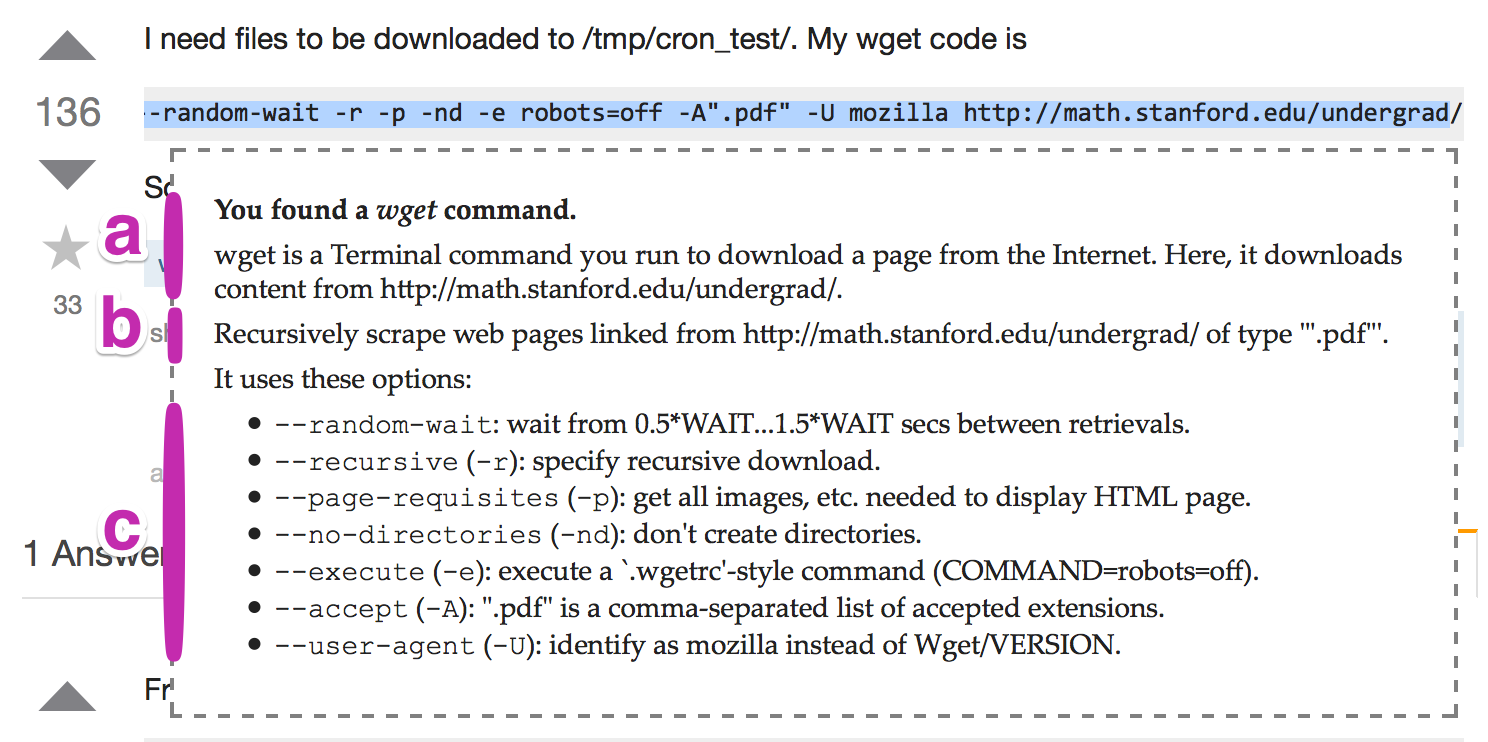
\includegraphics[width=\linewidth]{figures/tutorons_microexplanation}
    \caption{%
      A micro-explanation for a command line generated by a Tutoron with multiple levels of detail 
      (definition, high-level intent, arguments)
    }\label{fig:tutorons_microexplanation}
  }%
  \qquad
  \parbox{.45\textwidth}{%
    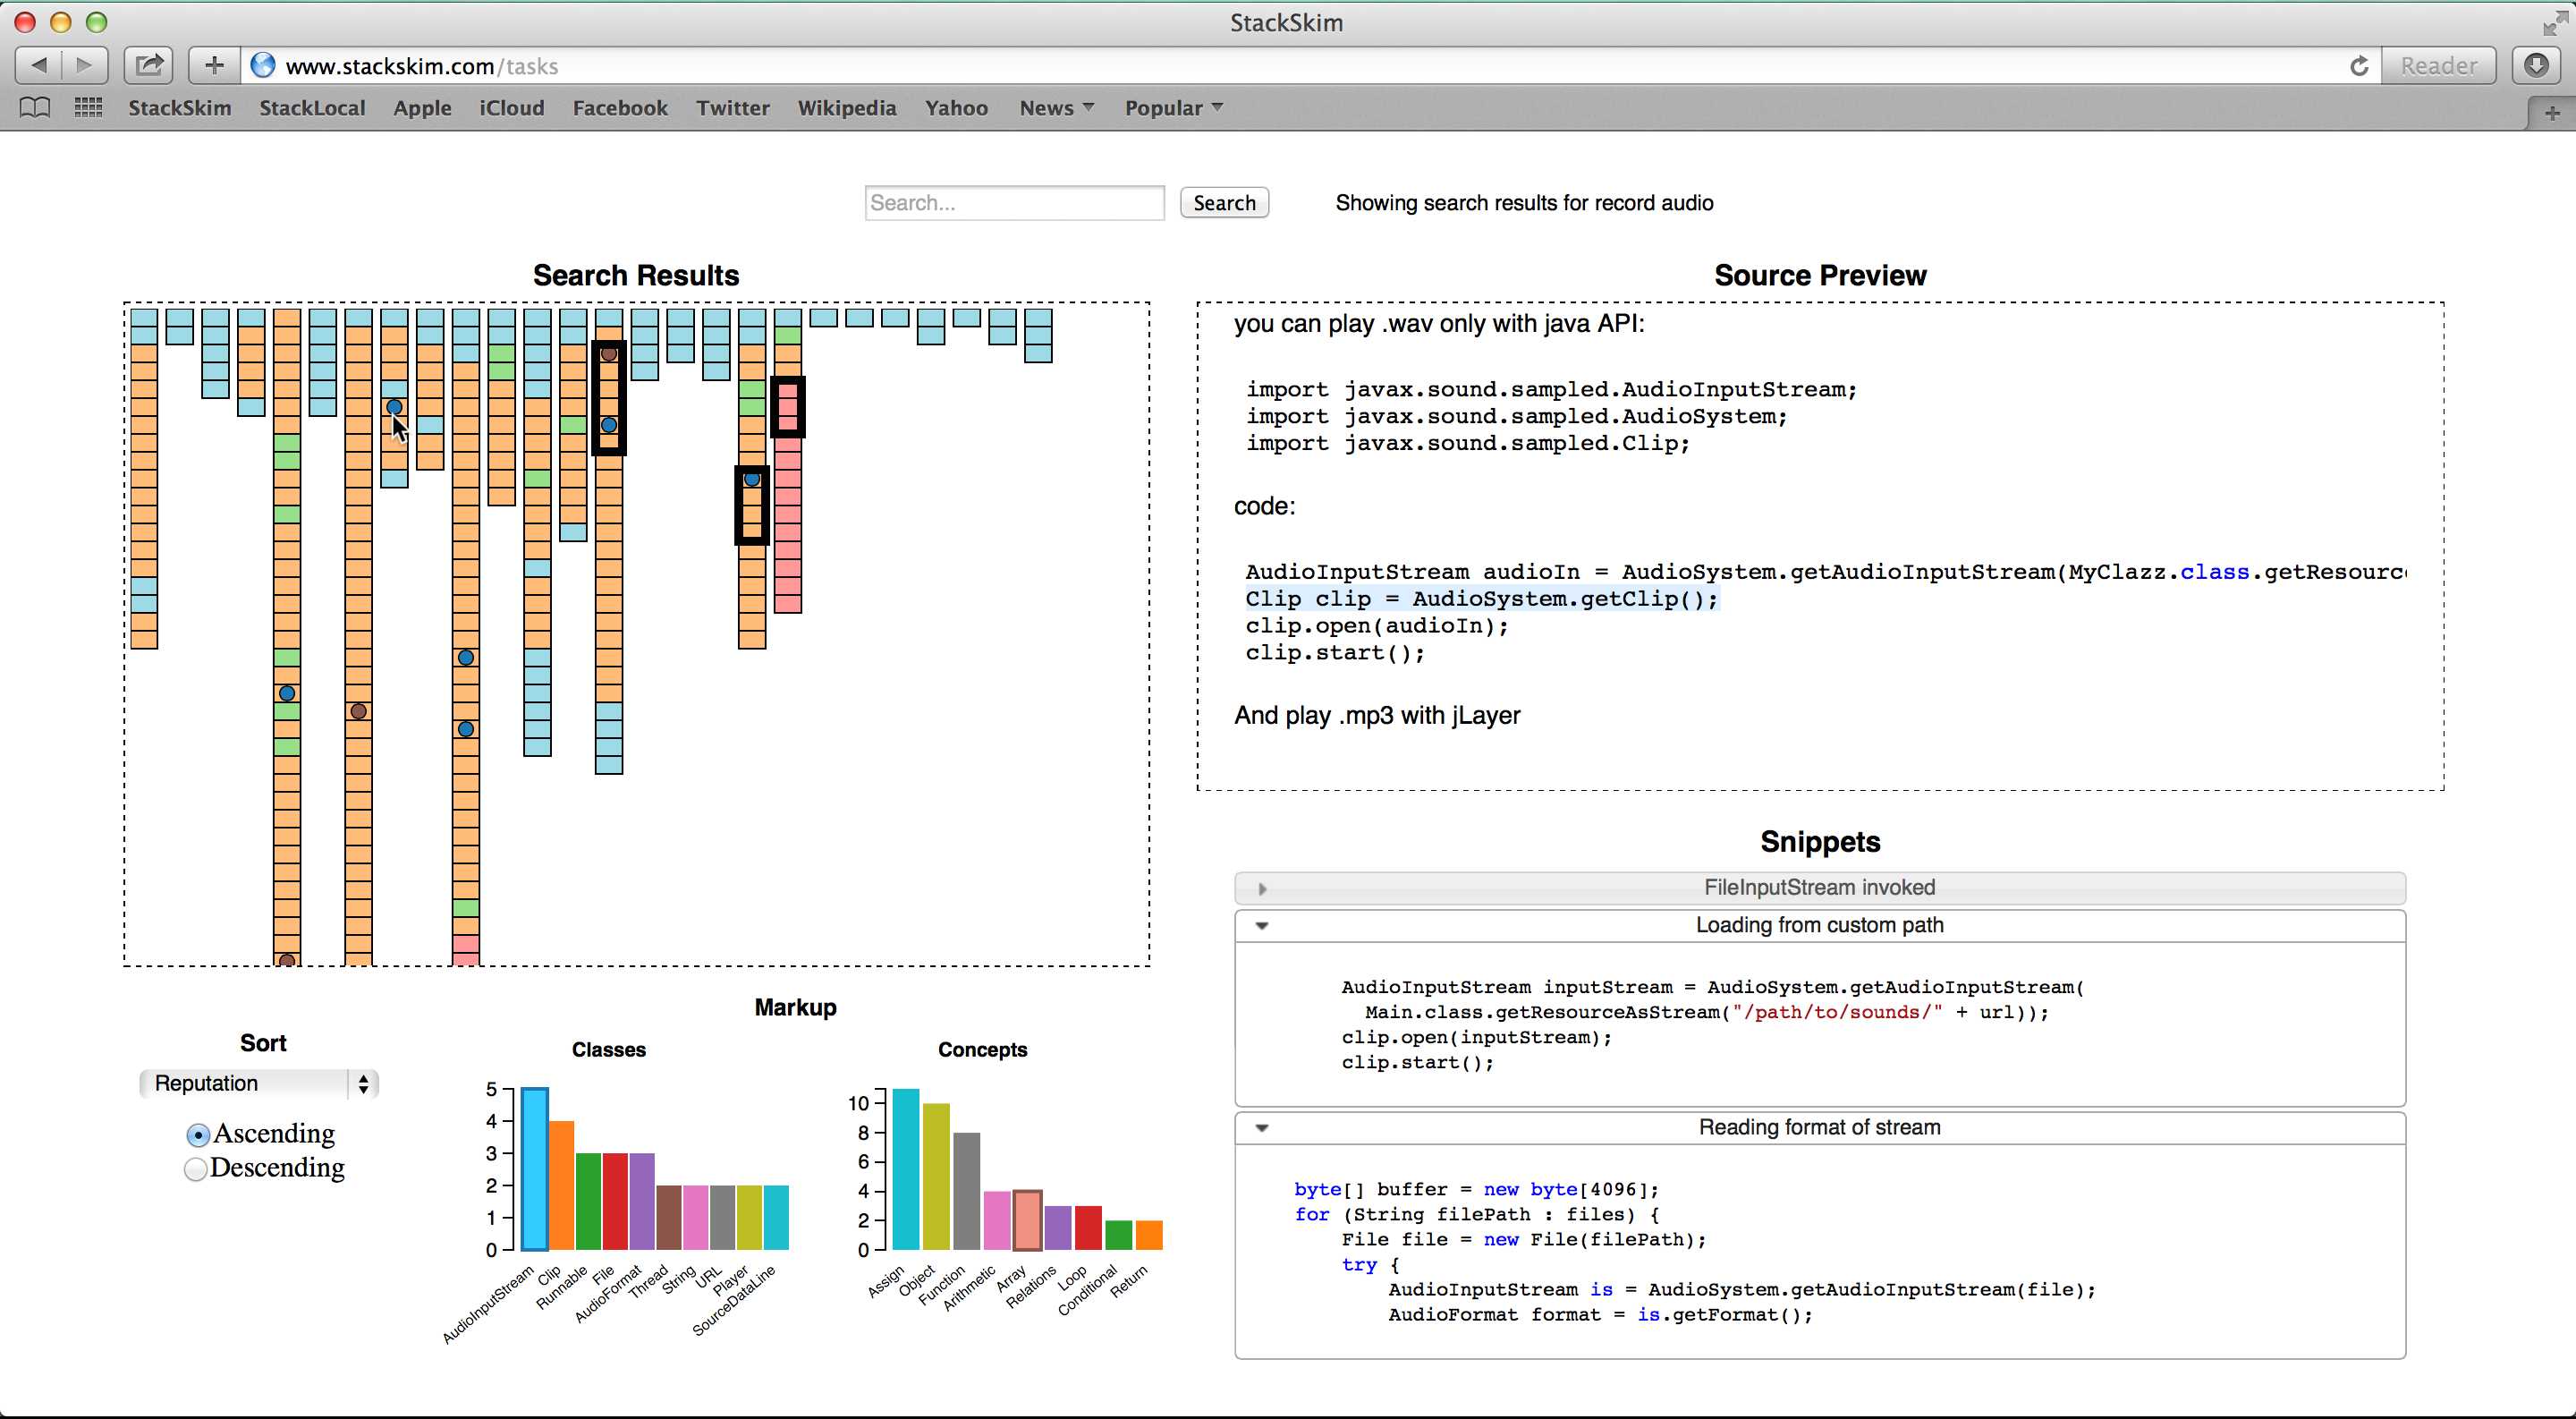
\includegraphics[width=\linewidth]{figures/stackskim_ui}
    \caption{%
      StackSkim, a visual interface for comparing and noticing trends in large collections of code examples that solve the same problem.
    }\label{fig:stackskim_ui}
  }
\end{figure}
\fi

\if 0
Point out the number of non-professional programmers.
Also point out crises in developing technologies that are caused by programmers who followed non-systematic practices

This work can be seen as an effort to reconcile the best practices of the ``systematic developer'' with recent tendencies of ``opportunistic'' programming habits.
\textbf{I could add in a mention of Blackwell's Attention Investment model here to mention why it is that programmers may program opportunistically, and why we should and how we can vary incentives and costs.}
Clarke introduced the persona of an \emph{opportunistic developer} to describe a software developer who writes code in an ``exploratory fashion'' and develops a ``sufficient understanding of a technology to understand how it can solve a business problem''.
(This contrasts with the \emph{systematic developer}, who writes code defensively and ``develops a deep understanding of a technology before using it''~\cite{clarke_what_2007}.)
In their study of exhibit designers at San Francisco's Exploratorium interactive science museum, Brandt et al.\ reported on a group who engaged in \emph{opportunistic programming} who weren't professional developers~\cite{brandt_opportunistic_2008} but were very much what might be considered as end-user programmers --- those developing code for personal rather than public use~\cite{ko_state_2011}.

Brandt et al.\ associated several habits with opportunistic programming that are counter to what we would hope for students working with code or end-users developing a better understanding of code.
Those programming opportunistically likely to incorporate functionality by copying and pasting code, often from online sources~\cite{brandt_two_2009}.
They are more likely to implement functionality from scratch for well-known libraries, instead of reusing existing systems and libraries~\cite{brandt_opportunistic_2008}.
They also practice ``code satisficing'', implementing functionality in a sub-optimal way in order to maintain flow and move on to other functionality~\cite{brandt_opportunistic_2008}.

While opportunistic programming is powerful in that it allows one to rapidly prototype and ideate and that it reduces the cycle time of editing and debugging code~\cite{brandt_opportunistic_2008}, this behavior discourages the formation of new mental models and an introduction to new tools that should be encouraged for both novice programmers and many end-user programmers.
The author of this proposal observed much of what would be called ``opportunistic'' habits while instructing a user interface design course.
After providing reference code to students for programming interfaces on Android phones and smartwatches, he helped students debug problems related to API reuse and the side effects of mixed code from multiple examples after hearing students self-report to having ``copied and pasted'' code from online tutorials and the slides he distributed.
In light of a prevalence of the ease of opportunistic habits and programmers' ability to copy-and-paste code from an increasingly comprehensive body of crowd documentation online~\cite{parnin_crowd_2012}, I define the goals of my research:

\emph{In my research, I develop and study software artifacts to support systematic inspection of found code from information interfaces programmers use when developing opportunistically.}

The theoretical deliverables of this work is establishing how systematic habits amidst opportunistic practice will improve:
(\emph{a}) programmers' mental models of reused code, libraries and tools used they develop
(\emph{b}) enable more accurate feasibility assessments of upcoming tasks (for example, see~\cite{ko_role_2011})
(\emph{c}) reduce design barriers~\cite{ko_six_2004} when planning new functionality

The artifacts that I develop belong to two themes:
\begin{itemize}[noitemsep]
\item Techniques for automatically generating instructive explanations and demonstrations of found code
\item Interfaces for critical inspection of alternatives when selecting code for reuse
\end{itemize}

I have developed the artifacts that enable exploration within both of these themes, and have published a first paper on the one of the two themes.
Toward the first, a paper I presented at VL/HCC explored techniques for automatically augmenting code in online examples with natural languages explanations and demonstrations of code.\footnote{%
The Tutorons system was implemented as both a browser plugin and a standalone JavaScript library, and can be viewed in action on \url{www.tutorons.com}.
}
We put forward a set of four guidelines to inspire the development of context-sensitive help:
(\emph{a}) leverage multiple representations to illuminate high-level intent and enable low-level understanding of syntax
(\emph{b}) be concise --- skip static explanations and focus on dynamically generated content
(\emph{c}) reappropriate existing documentation
(\emph{d}) inspect code examples on a large scale to support explanations of common usage.
In a nine-participant user study, the system was shown to reduce the number of accesses to external documentation needed to modify online code to perform new tasks.
\textbf{Next steps will include \ldots}
\textbf{Mention the theories used: MLT, layered documentation, Attention Investment}

Towards the second goal, I and co-developer have built a visual search interface for StackOverflow, a popular online programming Q\&A.
In response to Brandt et al.'s recommendations to develop tools that support ``comparing, reasoning about, integrating, and modifying found code''~\cite{brandt_opportunistic_2008}, we developed StackSkim, \emph{a visual search interface for exploring answers to StackOverflow questions that have a multitude of answers}.
The interface offers rapid visual inspection of frequent libraries used for addressing the searcher's programming problem;
through direct manipulation, users can also rapidly collect and compare similar code snippets.
\textbf{Next steps will include \ldots}

Each of these efforts relies on the cultivation of new software artifacts to aid programmers in understanding code during an opportunistic programming task.
Each has already followed and will continue to follow a mixed methods approach of observation and controlled experiments to determine how these tools indeed alter not only the task of opportunistic programming, but also programmers' behavior in selecting, understanding, and using code found online.
We are currently developing a version of Tutorons explanations that we hope will be incorporated into an introductory CS classroom's online textbook to better understand the role of automatic explanations of code for novice programmers.
\textbf{Add some note here about how we intend to run some workshop on clean code reuse habits.}
\fi

\section{References}
\printbibliography[heading=none]

\end{document}
